\chapter{Wind Tunnel Testing and Model Tuning}
\label{ch:windTunnel}

This chapter describes the wind-tunnel testing of MARGE and the tuning of the aeroservoelastic model to match the experimental data.

%%%%%%%%%%%%%%%%%%%%%%%%%%%%%%%%%%%%%%%%%%%%%%%%%%%%%%%%%%%%%%%%%%%%
\section{Data Acquisition and Analysis} %%%%%%%%%%%%%%%%%%%%%%%%%%%%
%%%%%%%%%%%%%%%%%%%%%%%%%%%%%%%%%%%%%%%%%%%%%%%%%%%%%%%%%%%%%%%%%%%%

MARGE's response was tested at the University of Washington's 3x3 low-speed wind tunnel. It was tested at six flight conditions, $q_D=\{60,100,163,207,281,343\}$ Pa. At each flight condition, the response to each of the four inputs was tested three times. For the gust vanes, a discrete 4-degree doublet gust was generated with a frequency of 1.45 Hz (approximately equivalent to the first wing bending natural frequency). For the ailerons, a 5-degree frequency sweep from 1 Hz to 2 Hz was performed. For the elevator, a 2-degree frequency sweep from 1 Hz to 2 Hz was performed. This frequency band was chosen as it encompassed the first wing bending mode and also stayed within the bandwidth of the actuators.

The exception to the above is at $q_d=343$ Pa. At this dynamic pressure, the aileron sweeps were reduced in magnitude to 3.5 degrees and the elevator sweep was reduced in magnitude to 1 degree. This was done in order to reduce the risk of damage to the model due to violent responses at high speeds. <verify with john>

All of these tests were controlled and recorded using Simulink Real-Time. The testing yielded time-series data of input commands and sensor readings for each test.

\subsection{Data Postprocessing}
The time-domain data was post-processed in a similar way as was done for the GVT data in Section \ref{sec:generateFRF}. Each run's data was truncated to start when the input began and end five seconds after the input ended. The data was re-centered to have zero mean and then the three runs of each test were concatenated.

This single concatenated time-domain signal was then buffered into overlapping Hann windows and transformed using the CZT. The FRFs were then computing using Equation \ref{eq:frf}.

\subsubsection{Accelerometer Data Postprocessing}

issues will be further discussed in the next chapter <insert>

bandwidth out [1,2] <insert>

bandpass in [0.8,25] <insert>

re-center <insert>


%%%%%%%%%%%%%%%%%%%%%%%%%%%%%%%%%%%%%%%%%%%%%%%%%%%%%%%%%%%%%%%%%%%%
\section{Model Tuning} %%%%%%%%%%%%%%%%%%%%%%%%%%%%%%%%%%%%%%%%%%%%%
%%%%%%%%%%%%%%%%%%%%%%%%%%%%%%%%%%%%%%%%%%%%%%%%%%%%%%%%%%%%%%%%%%%%

The state-space model generated in Chapter \ref{ch:sysModeling} was adjusted such that its frequency response fit the experimental frequency response. This was done by adjusting certain parameters in the model that each represented some uncertainty in the model's physical characteristics. This adjustment was first done by hand, and then repeated in a automated process through optimization.

\subsection{Tuning Parameters} %%%%%%%%%%%%%%%%%%%%%%%%%%%%%%%%%

The state-space model derived in Chapter \ref{ch:sysModeling} assumes linear structural dynamics, linear aerodynamics, and thin airfoils. It also requires perfect knowledge of mode shapes. In reality, MARGE does not conform to any of these assumptions perfectly. Thus, tuning parameters were implemented in the state-space model generation script which adjusted the structural and aerodynamic modeling to compensate.

The first tuning parameter is the first wing bending natural frequency $\omega_{n,2}$. This quantity has a low uncertainty, but was treated as a tuning parameter for purposes of investigation.

The next tuning parameters are the damping ratios $\zeta$ for the modes. These have higher uncertainty since viscous damping is not the most physically accurate model for structural damping. Furthermore, aerodynamic damping of motions is not accounted for in the model. These can be compensated for by adjusting the damping ratios with this tuning parameter.

The next tuning parameters are the effectiveness $\tau$ of the controls. Each control surface will not be as effective as predicted by the linear aerodynamic model due to airfoil thickness, viscous effects (such as flow separation), roughness, and gaps in construction. These can be compensated for by adjusting the control effectiveness of each control surface. These tuning parameters scale the forces predicted for the control surfaces by the linear aerodynamic model.

The final tuning parameters are scaling factors $\tau_{P_{ss}}$ for each entry of $[P_{ss}]$. (Refer to Eq. \ref{eq:EOMwRoger} for the context in which $[P_{ss}]$ is used in modeling.) These scale the lift of the lifting surfaces (not including the control surfaces) to account for airfoil thickness, viscous effects, roughness, and gaps in construction.

A summary of tuning parameters and their default values (which apply no correction) is shown in Table \ref{tab:tuningParams}. The comparison of this initial un-tuned model's FRFs and the experimental FRFs can be seen in Fig. \ref{fig:noTuneFRF}.
\begin{table}[h]
	\centering
	\label{tab:tuningParams}
	\caption{Default Values of MARGE Tuning Parameters}
	\begin{tabular}{ccc}
		\hline\hline
		Name & Default Value & Description \\
		\hline
		$\omega_{n,2}$ & 1.4544 & first wing bending mode frequency \\
		$\zeta_1$ & 0 & rigid pitching damping ratio \\
		$\zeta_2$ & 0.028 & first wing bending damping ratio \\
		$\tau_\text{ail1}$ & 1 & aileron 1 effectiveness \\
		$\tau_\text{ail2}$ & 1 & aileron 2 effectiveness \\
		$\tau_\text{elev}$ & 1 & elevator effectiveness \\
		$\tau_\text{gust}$ & 1 & gust vane effectiveness \\
		$\left[\tau_{P_{ss}}\right]$ & all ones & lift scaling \\
		\hline\hline
	\end{tabular}
\end{table}

\begin{landscape}

\begin{figure}[H]
	\centering
	\label{fig:noTuneFRF}
	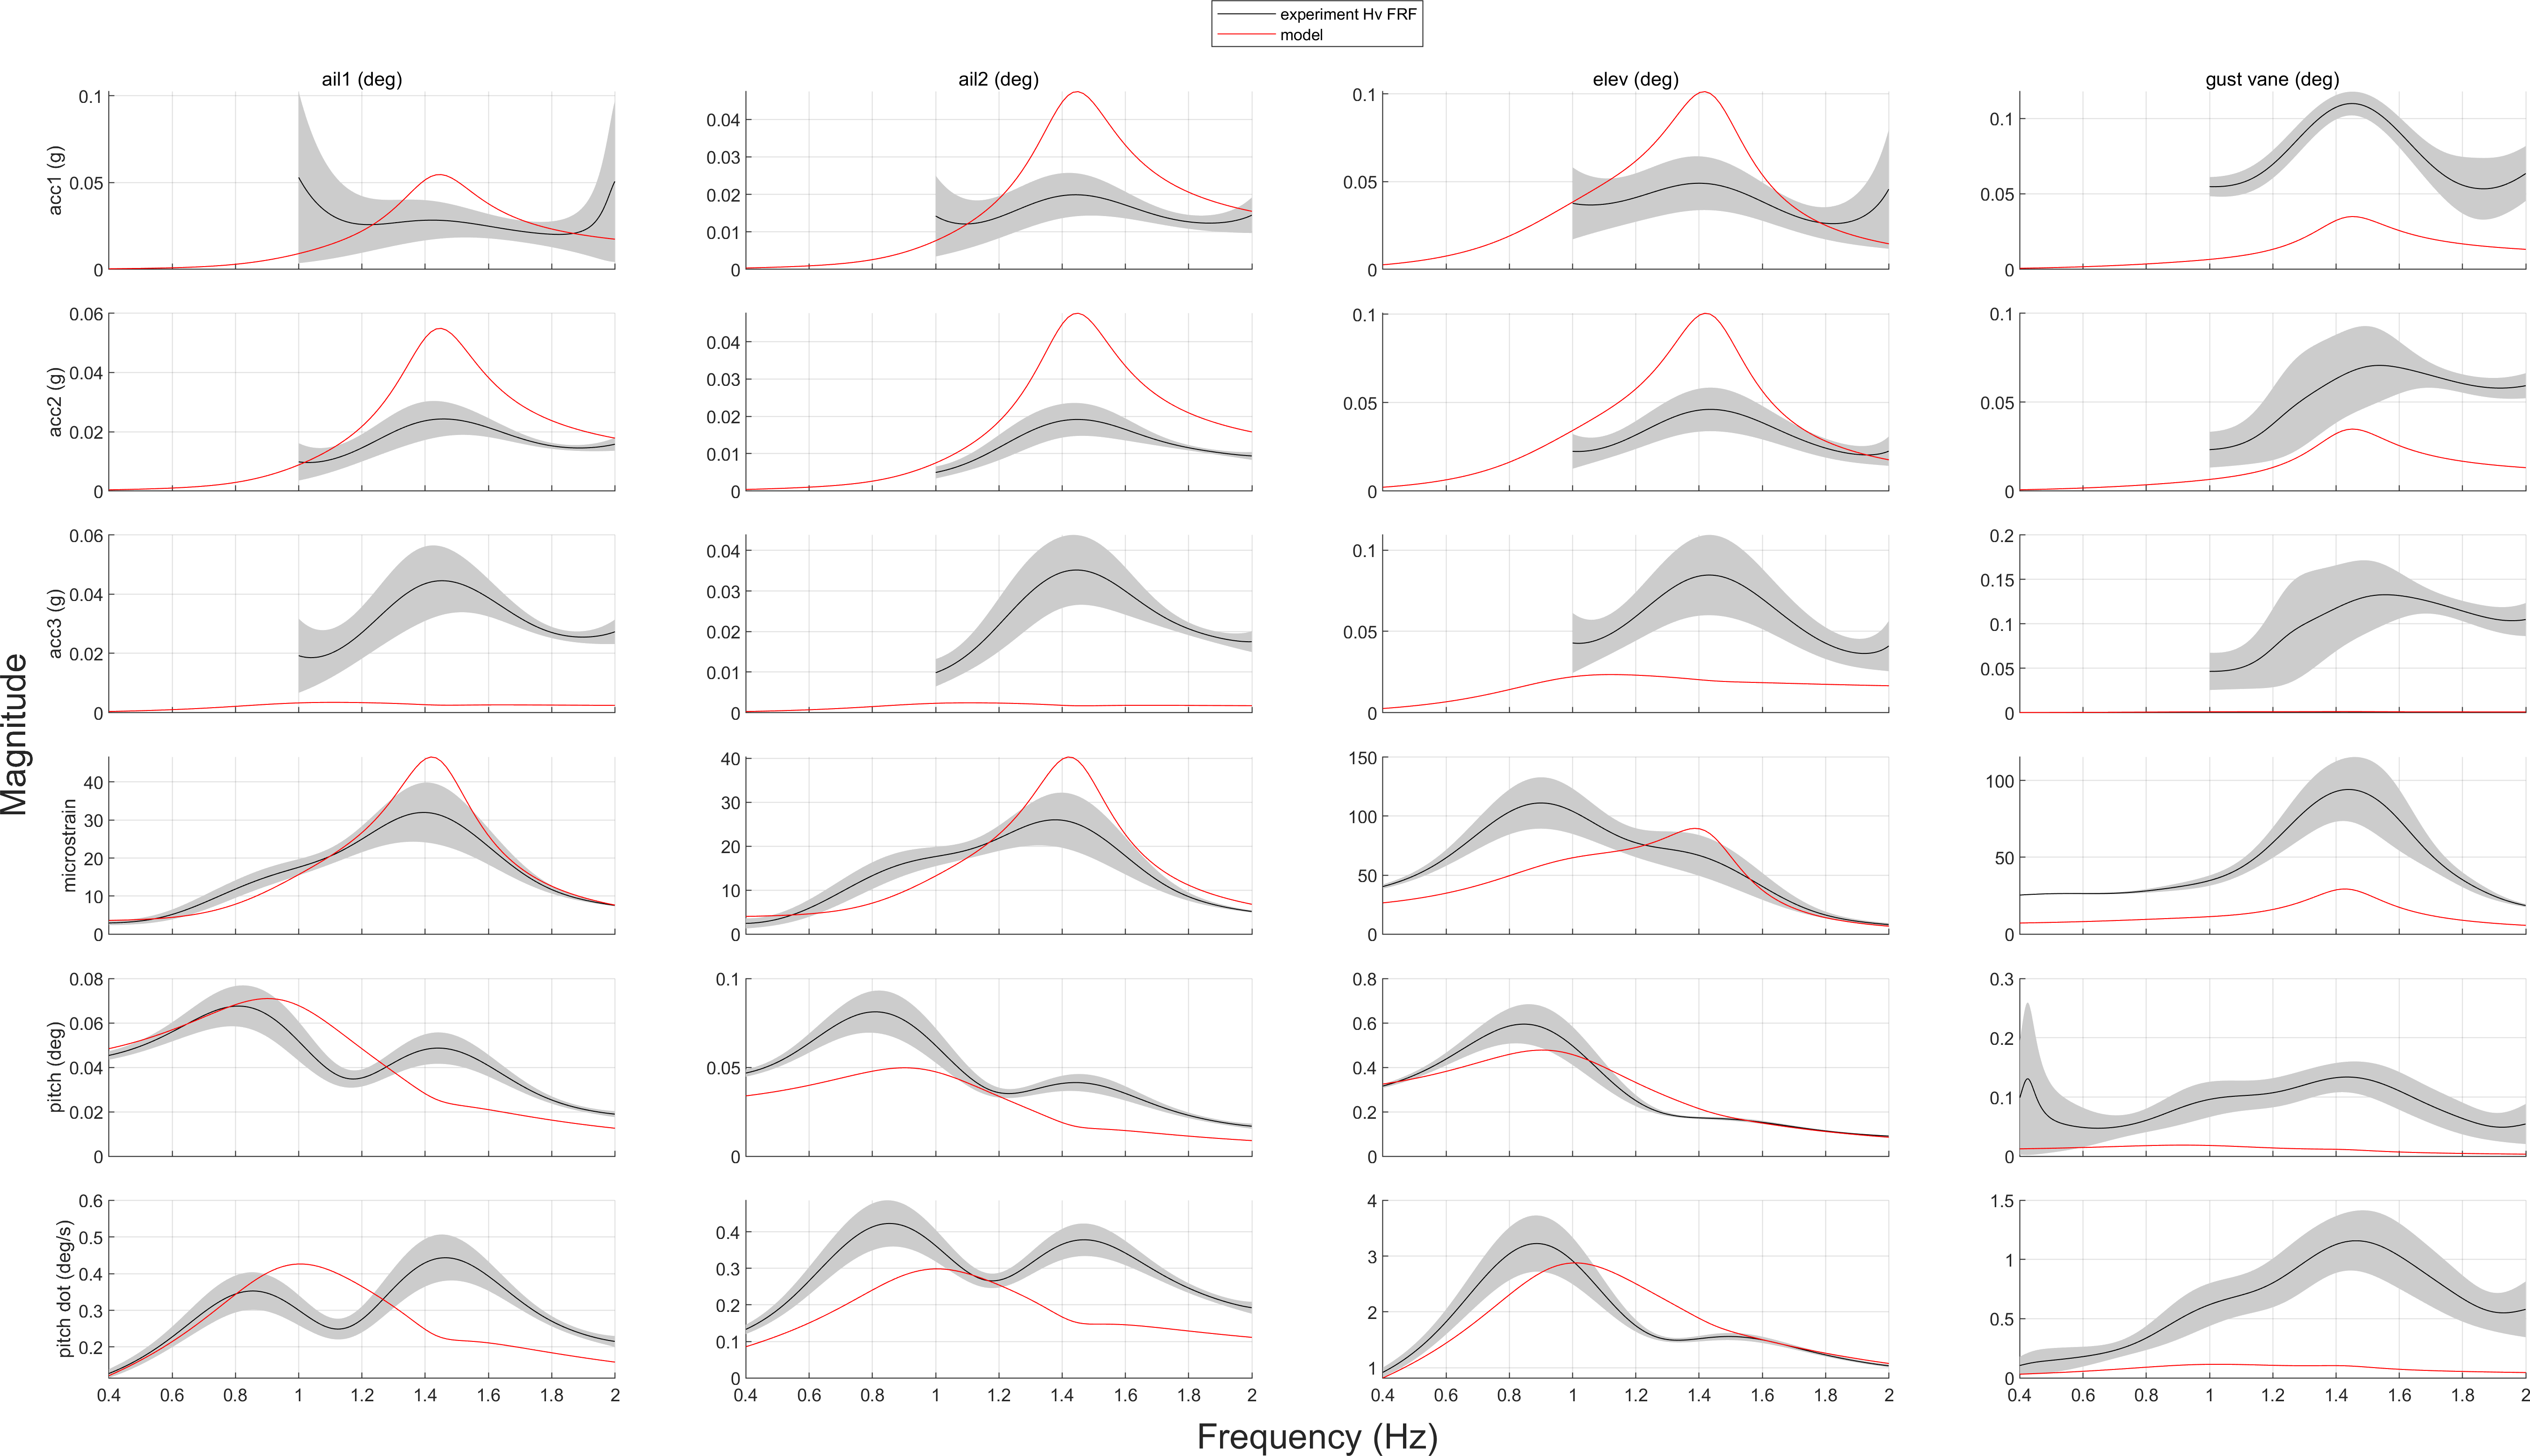
\includegraphics[width=9in]{figs/FRFcompare_noTune_q207.png}
	\caption{A comparison of experimental FRFs and untuned model FRFs. The grey region is enclosed by the $H_1$ FRF below and the $H_2$ FRF above of the experimental data.}
\end{figure}

\end{landscape}



\subsection{Manual Model Tuning} %%%%%%%%%%%%%%%%%%%%%%%%%%%%%%%

The first step in tuning was experimenting with manual changes to the tuning parameters with the goal of closing the gap between the model's FRF and the experimental FRF. This was done by thinking intuitively about the modeling uncertainties which are most likely effecting the known discrepancies in the FRFs. For example, it was known that linear aerodynamics would overpredict the control surface effectiveness by up to 50\% even in reasonably small ($<10^\circ$) deflections \cite{young1947,riebe1955}. Thus, the control effectiveness of the ailerons and elevator were lowered until the FRFs with these controls as inputs better matched the experimental FRFs in magnitude.

The resultant parameters and FRF comparison of the manually tuned model are shown below in Table \ref{tab:manualTuning} and Fig. \ref{fig:manualTunedFRF}. The poor fit in Fig \ref{fig:manualTunedFRF} indicates that the simple and ``intuitive'' manual tuning is not sufficient to completely match the experiment.
\begin{table}[h]
	\centering
	\label{tab:manualTuning}
	\caption{Manually Tuned Values of MARGE Tuning Parameters}
	\begin{tabular}{ccc}
		\hline\hline
		Name & Default Value & Adjusted Value \\
		\hline
		$\omega_{n,2}$ & 1.4544 & N/A \\
		$\zeta_1$ & 0 & 60 \\
		$\zeta_2$ & 0.028 & N/A \\
		$\tau_\text{ail1}$ & 1 & 0.6 \\
		$\tau_\text{ail2}$ & 1 & 0.7 \\
		$\tau_\text{elev}$ & 1 & 0.6 \\
		$\tau_\text{gust}$ & 1 & N/A \\
		$\left[\tau_{P_{ss}}\right]$ & all ones & $\begin{bmatrix} 0.9 & 1 \\ 0.5 & 1.5 \end{bmatrix}$ \\
		\hline\hline
	\end{tabular}
\end{table}

\begin{landscape}

\begin{figure}[H]
	\centering
	\label{fig:manualTunedFRF}
	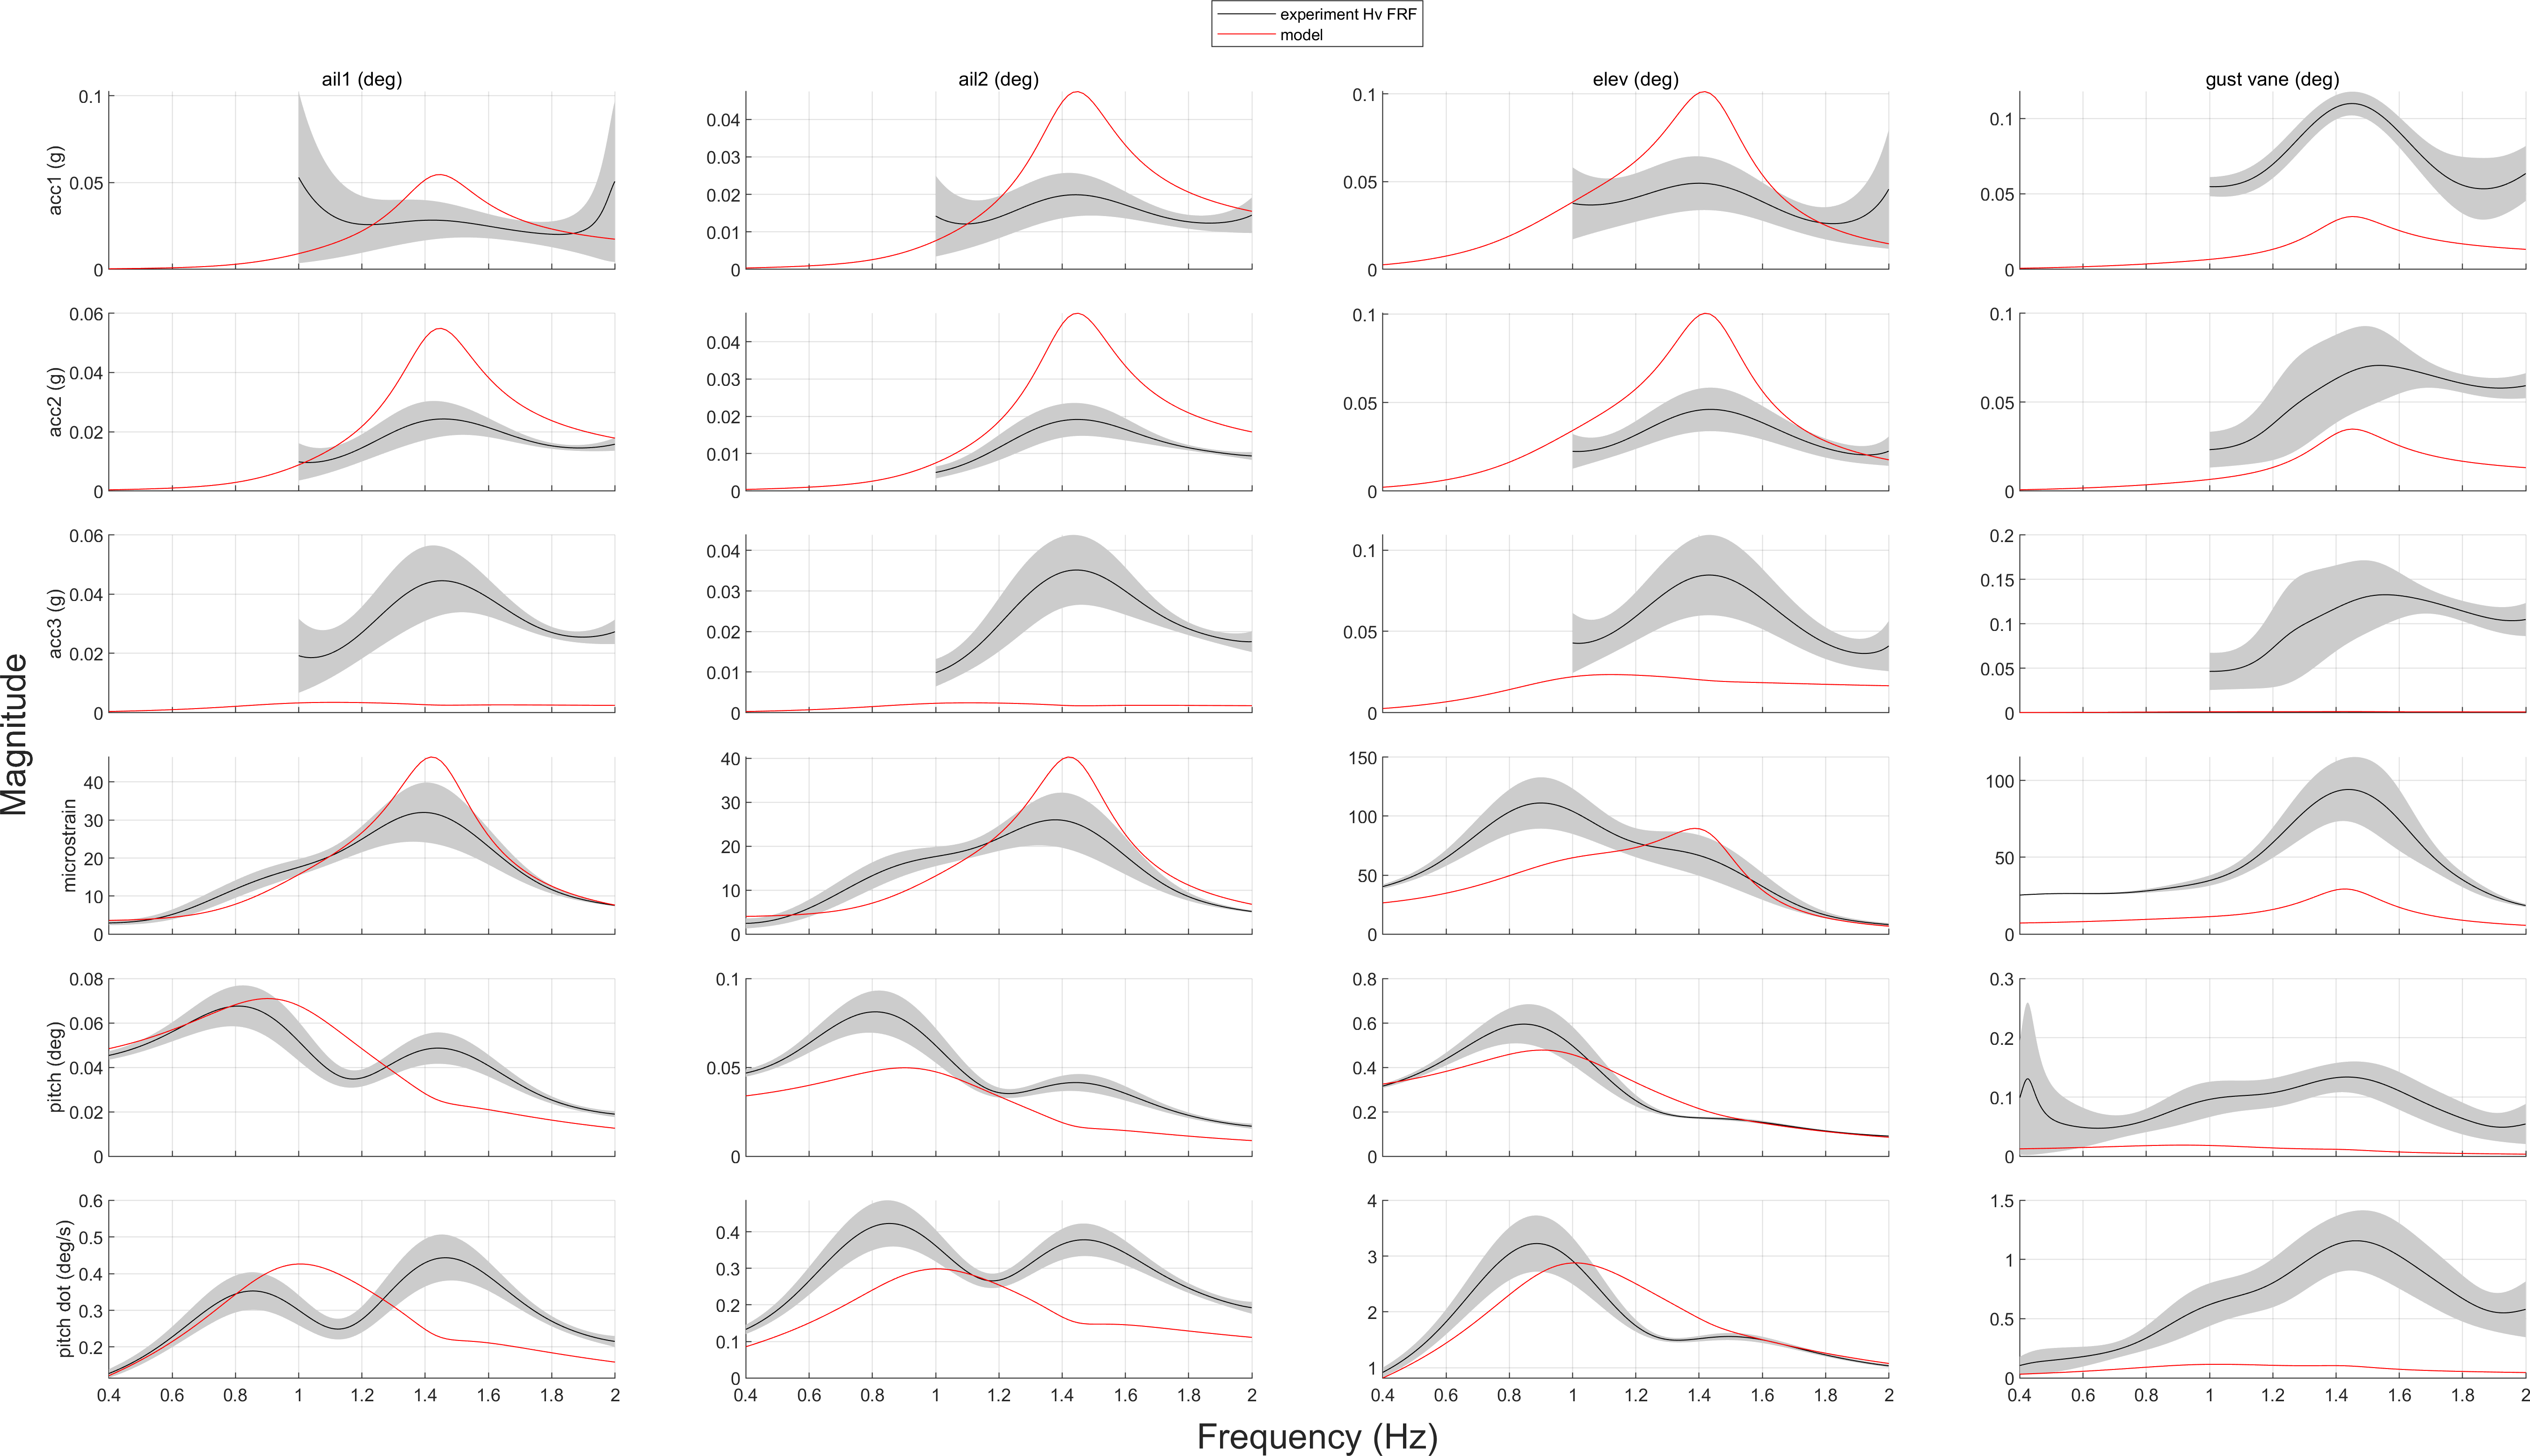
\includegraphics[width=9in]{figs/FRFcompare_manualTune_q207.png}
	\caption{A comparison of experimental FRFs and manually-tuned model FRFs. The grey region is enclosed by the $H_1$ FRF below and the $H_2$ FRF above of the experimental data.}
\end{figure}

\end{landscape}

\subsection{Model Optimization} %%%%%%%%%%%%%%%%%%%%%%%%%%%%%%%%


obj
\begin{align}
	F(\{x\}) &= \sum_{i=1}^{N_\text{in}} \sum_{j=1}^{N_\text{out}} f_{i,j}(\{x\}) \\
	f_{ij}(\{x\}) &= \epsilon_{ij \, \text{mag}} \sqrt{\lambda} + \epsilon_{ij \, \text{phase}} \frac{1}{\sqrt{\lambda}}
\end{align}
\begin{align}
	\epsilon_{ij \, \text{mag}} &= \sum_\omega \frac{|FRF_\text{exp} (\omega)| - |FRF_\text{model} (\omega)|}{|FRF_\text{exp} (\omega)|} \\
	\label{eq:phaseCompare}
	\epsilon_{ij \, \text{phase}} &= \sum_\omega \left( \angle FRF_\text{exp} (\omega) - \angle FRF_\text{model} (\omega) \right)
\end{align}
%The actual implementation of Eq. \ref{eq:phaseCompare} is augmented with a modulo operator to take the lowest phase difference between the experimental data point and the model data point. This avoids artifacts in phase measurements due to numerical computation of phase. Thus, $\epsilon_{ij \, \text{phase}}$ is more robustly computed as
%\begin{align}
%	\epsilon_{ij \, \text{phase}} &= \sum_\omega \left( \angle FRF_\text{exp} (\omega) - \angle FRF_\text{model} (\omega)
%\end{align}